\documentclass[sigconf,anonymous,review]{acmart}

\acmConference[WSDM '27]{The 20th ACM International Conference on Web Search and Data Mining}{February 2027}{Hong Kong}
\settopmatter{printacmref=false}
\renewcommand\footnotetextcopyrightpermission[1]{}
\pagestyle{plain}

\usepackage{booktabs}
\usepackage{multirow}
\usepackage{xcolor}
\usepackage{pgfplots}
\pgfplotsset{compat=1.17}

\begin{document}

\title{Detection Is Not Actionability: When Should LLM Query Expansion Be Applied?}

\author{Anonymous Author(s)}
\affiliation{\institution{Affiliation withheld for double-blind review}}

\begin{abstract}
LLM query expansion can improve retrieval, but applying it
unconditionally also harms a measurable fraction of queries. A natural
response is to apply it selectively: expand only queries where
retrieval is predicted to be failing. We test this directly. Qrel-free
retrieval telemetry, recorded before any action, is a reasonably
effective detector of retrieval failure (AUC $0.649$ on TripClick
TAIL test, replicating at $0.680$ on an independent BEIR Natural
Questions split). The same kind of telemetry, recorded after a specific
expansion action, is markedly worse at predicting whether that action
helped (AUC $0.552$ on TripClick, $0.556$ on NQ) --- a statistically
significant gap on both corpora. We then test the obvious consequence:
does routing expansion on the easier signal alone, a failure-selective
controller, recover selective-QE's promise? It does not: the
failure-selective policy's point estimate is the best of three real
policies tested, but is not significantly different from unconditional
expansion, from doing nothing, or from a more expensive closed-loop
agent that also consults post-action telemetry. Detecting that
retrieval needs help is not the same problem as knowing what will
actually help it, and the gap between the two is where selective query
expansion's promise currently stalls.
\end{abstract}

\maketitle

\section{Introduction}

Large language models can generate useful pseudo-documents,
alternative phrasings, and disambiguating context for a search query,
and corpus-grounded expansion --- conditioning the rewrite on
retrieved evidence rather than the query alone --- improves on naive
query-only rewriting. But LLM query expansion (QE) applied
unconditionally can also be net-harmful on a measurable fraction of
queries, particularly ones that are already well served or already
underspecified in a way expansion cannot fix. Existing work establishes
that QE \emph{can} help; it leaves open when a system should trust an
expansion enough to apply it, and in practice QE is deployed either
unconditionally or not at all.

The natural fix is selective expansion: identify queries where
retrieval is already failing, and expand only those. This requires two
different predictive judgments, which prior query-performance-prediction
and selective-expansion work has not clearly separated:

\[
\underbrace{P(\text{retrieval failure} \mid x)}_{\text{detection}}
\quad\neq\quad
\underbrace{P(\Delta\text{nDCG} > 0 \mid x, a)}_{\text{actionability}}
\]

Detection asks whether something is already wrong. Actionability asks
whether a \emph{specific} intervention will fix it. A system could
answer the first question well and the second poorly, in which case
selective expansion gated on detection alone would not actually
recover expansion's promise --- it would route the right queries to an
intervention whose benefit is still a coin flip.

\textbf{Research question.} Can retrieval telemetry that identifies
poorly served queries also determine when LLM query expansion should
be applied?

\textbf{Contributions.}
\textbf{(C1) Detection $\neq$ actionability.} Pre-action retrieval
telemetry identifies failing retrieval significantly better than
post-action telemetry predicts whether a specific QE action helped,
replicating on an independent second corpus.
\textbf{(C2) Detection alone does not solve selective QE.} A
failure-selective controller built directly on the stronger signal has
the best point estimate of the policies tested, but does not
significantly outperform unconditional QE, BM25 alone, or a more
expensive closed-loop agent.
\textbf{(C3) The gap is not corpus-specific.} TripClick's
detection-vs-actionability ordering ($0.649$ vs.\ $0.552$) replicates
on BEIR Natural Questions ($0.680$ vs.\ $0.556$), an open-domain
corpus unrelated to TripClick's clinical queries.

\section{Related Work}

\textbf{LLM query expansion.} Query2doc~\cite{query2doc} generates
pseudo-documents from an LLM and appends them to the query; MuGI
\cite{mugi} generates and fuses multiple expansions. Both treat
expansion as unconditional, one-shot generation, conditioning on
neither retrieval-state telemetry nor a harmful rewrite's
recoverability. Query2doc's pseudo-documents are generated purely from
the LLM's parametric knowledge via few-shot prompting, with no
retrieval step in generation itself; our expansion is corpus-grounded
instead --- conditioned on retrieved evidence rather than the query
text alone --- and this generation mechanism is held fixed across all
four policies, so what varies across Table~\ref{tab:policies} is only
\emph{whether} and \emph{when} it fires, not the mechanism itself.

\textbf{Query performance prediction and selective expansion.} Classic
query performance prediction~\cite{qpp-clarity} and selective query
expansion~\cite{selective-qe} ask whether a query is hard, or likely to
benefit from expansion, from retrieval signal alone --- the same
underlying question as our detection task. Neither separates that
question from the distinct, harder one of whether a \emph{specific}
candidate action will help: prior selective-QE evaluations report
whether expansion was gated well in aggregate, not whether the gating
signal and the treatment-effect signal are the same predictive problem
or two different ones of differing difficulty. We make that separation
explicit and test it directly.

\textbf{Selective rewriting and adaptive retrieval.} Two recent,
independent studies reach a conclusion consistent with ours through
different mechanisms. Abe et al.~\cite{qe-fails-unfamiliar} show LLM
QE degrades retrieval specifically when the model lacks query
knowledge or the query is ambiguous --- evidence that unconditional
expansion's harm is systematic, not noise, reinforcing why selective
gating is worth attempting in the first place. Kotte~\cite{not-all-queries-need-rewriting}
tests selective gating directly: on three BEIR domains with dense
retrievers and prompt-only (non-grounded) rewriting, a feature-based
gate achieves AUC $0.593$ and does not reliably beat never-rewriting,
with an oracle ceiling of only $+3$pp ($6\%$ relative). This
corroborates our Result 2 on an unrelated retrieval stack, rewriting
mechanism, and domain set, strengthening the case that the difficulty
is general rather than an artifact of either study's setup. Neither
that work nor Adaptive-RAG~\cite{adaptive-rag}, which routes queries
to a retrieval depth using a learned complexity classifier validated
only on end-to-end accuracy, separately measures whether a gating
signal's own detection accuracy matches its accuracy at predicting the
chosen intervention's benefit. We make that decomposition explicit,
quantify the gap directly as two different AUCs, and show it is
significant and replicates across two further corpora.

\section{Selective Query Expansion Setup}

\textbf{Datasets.} TripClick~\cite{tripclick} is the primary benchmark:
1{,}523{,}878 documents, split into head/torso/tail query-frequency
buckets, each with train/validation/test splits (1{,}175 queries per
split per bucket); we report the TAIL split, click-derived labels.
BEIR Natural Questions~\cite{beir,natural-questions} is an independent
replication corpus, open-domain and unrelated to TripClick's clinical
queries, with no native train/val/test partition; we carve a disjoint,
fixed-seed (42) split ourselves (800 validation) and fit fresh
detectors, never reusing TripClick's weights. An initial $n{=}600$
pilot touch of test was directionally consistent with TripClick but
too imprecise to resolve the AUC ordering on its own; we then ran the
identical frozen pipeline, unchanged, as a single confirmatory test on
the entire remaining, disjoint pool of $2{,}052$ never-before-touched
NQ queries, reported here in full and never pooled with the pilot. The
extension's scope and stopping rule were committed in writing before
touching any of its data, precisely to foreclose the reading ``touched
test, saw an inconclusive number, expanded it.'' The $n{=}2{,}013$ in
Table~\ref{tab:headline} is this confirmatory set's acted-upon subset.

\textbf{Retrieval failure}, the detection target, is defined as BM25
returning zero relevant documents in its top 10 results for that
query --- a binary, click-derived judgment available without any
model predictions, fixed identically across both corpora.

\textbf{Policies compared.} All four share the same retriever,
grounding, and generator, differing only in when/whether QE fires:

\begin{center}
\small
\begin{tabular}{@{}ll@{}}
\toprule
Policy & Decision rule \\
\midrule
BM25 & Never expand \\
Static QE & Always expand \\
Failure-selective QE & Expand iff $P(\text{fail}\mid x) > \tau$ \\
Closed-loop QE & Expand, then accept/rollback on post-action telemetry \\
\bottomrule
\end{tabular}
\end{center}

$\tau$ is the median predicted failure probability on validation,
fixed before touching test, never swept or re-chosen against any
reported result. Failure-selective QE uses \emph{only} pre-action
telemetry; Closed-loop QE additionally consults post-action telemetry
through the same action-utility model as Result 1 (Section 4), scored
against thresholds calibrated on validation only: a sufficiently
positive score \emph{accepts} the rewrite via reciprocal-rank fusion
with the pre-action ranking, a sufficiently negative score
\emph{rolls back} to the pre-action ranking, and an ambiguous score
\emph{replans} with a different expansion operator, capped at two
generator calls per query.

\textbf{BM25 baseline validation.} A null result is only informative
if the baseline it is measured against is itself competitive --- an
under-tuned BM25 would make any intervention look falsely beneficial
by comparison. Our initial unstemmed BM25 scored nDCG@10 $0.228$ on
TripClick TAIL test, $15\%$ below the $0.267$ published reference for
this exact split and label type. Selecting entirely on validation,
Porter stemming and a $10{:}1$ title:body field weight close the gap
(validation nDCG@10 $0.235 \to 0.327$); a single confirmatory test
touch of the corrected configuration gives nDCG@10 $0.315$,
\emph{above} the published reference. All results in this paper use
this corrected baseline.

\textbf{Implementation.} Sparse retrieval is BM25 over a SQLite FTS5
index, reranked with
\texttt{cross-\allowbreak encoder/\allowbreak ms-marco-\allowbreak
MiniLM-\allowbreak L6-\allowbreak v2}~\cite{minilm-cross-encoder}, a
cross-encoder fine-tuned on MS MARCO passage ranking. Generation uses
\texttt{qwen2.5:3b}, 4-bit quantized (Q4\_K\_M), served locally via
Ollama with greedy decoding (temperature $0$), capped at two calls per
query episode with a $32$--$64$ token structured output --- the
language model is never the entire decision surface, only one typed
action within a small, fixed action space. All experiments run on a
single consumer machine (Apple M4 MacBook Air, 16GB unified memory),
no GPU cluster or cloud spend. All retrieval-config, detector, and
threshold decisions are made on validation only. Reported confirmatory
results use frozen configurations, with no subsequent model,
threshold, or retrieval decision conditioned on those outcomes;
earlier implementation-debugging accesses to test, from fixing two
apparatus defects mid-development, are disclosed and documented in the
supplementary repository rather than omitted. Significance throughout
is a paired bootstrap (10{,}000 resamples, seed $42$). Every number in
this paper is produced by a numbered, archived script in that
repository and is reproducible from frozen artifacts without rerunning
the generator: Table~\ref{tab:headline}'s AUCs and paired differences
from the frozen detection/calibration runs; Table~\ref{tab:policies}
and Section 6's oracle, selectivity-frontier, and failure-selective
figures from one shared frozen checkpoint, combined under each
policy's decision rule; and Section 6's validation-oracle robustness
check from a dedicated script that touches no test data.

\begin{center}
\small
\begin{tabular}{@{}ccc@{}}
\multicolumn{3}{c}{\textit{Retrieval telemetry}} \\[2pt]
\multicolumn{3}{c}{$\big\downarrow$} \\[2pt]
\textit{Failure detection} & \hspace{1cm} & \textit{Action utility} \\
``Is retrieval bad?'' & & ``Did QE help?'' \\
AUC $\mathbf{0.649}$ & & AUC $\mathbf{0.552}$ \\
\end{tabular}
\end{center}

\section{Result 1: Detection Is Easier Than Actionability}

A failure detector --- a logistic classifier on eight pre-action
retrieval-telemetry features (top retrieval score, score margin, score
entropy, query-term coverage, mean rare-term IDF, entity overlap,
lexical result coherence, and ranking stability under a small
controlled query perturbation) --- is moderately predictive of whether
retrieval has already failed (5-fold CV on validation, touched once on
frozen test). An action-utility model, observing a \emph{specific}
candidate action's consequences through ten post-action features
(score and coverage \emph{gains}, drift, reranker disagreement, and
reranker-specific signals the detector does not have access to) fit by
linear regression against the true nDCG change, is markedly weaker at
predicting whether that action helped. The action-utility model has
more features, including reranker signals entirely unavailable to the
detector, yet still under-performs it --- the gap in
Table~\ref{tab:headline} is not an artifact of the detector having a
richer or more favorable feature set. It is also not an artifact of
comparing a classifier against a regressor: refitting the
action-utility model directly as a logistic classifier on the same ten
features and the identical val/test protocol gives AUC $0.563$, 95\%
CI $[0.529,0.598]$ (\texttt{scripts/32}) --- indistinguishable from the
regression-based $0.552$ and still clearly below detection's CI on
this corpus, with no overlap. A non-linear model class does not close
it either: a gradient-boosted alternative was tried on this same
feature set during development and scored worse under 5-fold CV
(Pearson $r=0.045$ vs.\ $0.134$ for linear regression), so the deployed
model was never swapped in.

\begin{table}[h]
\caption{Detection vs.\ actionability AUC, both corpora. Both numbers
per corpus are frozen, evaluated once under the corpus's fixed
configuration.}
\label{tab:headline}
\small
\begin{tabular}{@{}lccc@{}}
\toprule
Task & TripClick & BEIR NQ & Difference \\
\midrule
Failure detection & 0.649 & 0.680 & --- \\
QE action utility & 0.552 & 0.556 & --- \\
\midrule
Paired difference & $+0.091$* & $+0.119$* & \\
\bottomrule
\end{tabular}
\\[2pt]
\footnotesize *: 95\% CI excludes zero (TripClick: $[+0.045,+0.136]$,
$n{=}1157$; NQ: $[+0.076,+0.162]$, $n{=}2013$).
\end{table}

The gap is not an artifact of comparing different noise levels: both
numbers per corpus come from the same features, protocol, and
population, and a paired bootstrap on the acted-upon subset confirms
the difference itself, not just non-overlapping point estimates. This
ordering --- pre-action telemetry beats post-action telemetry at
predicting intervention utility --- replicates on an open-domain
corpus unrelated to TripClick's clinical queries, providing evidence
that the ordering is not specific to TripClick.

\textbf{A bounded dense-retrieval pilot.} Both results above use BM25.
To check whether first-stage retrieval family matters, we ran a
bounded pilot substituting a dense bi-encoder
(\texttt{BAAI/\allowbreak bge-small-\allowbreak en-v1.5}~\cite{bge-embedding}) for BM25 on TripClick TAIL: 300
queries (150 val, 150 test, seed 42) against a scoped corpus (all
qrel-relevant documents for these queries plus $150$k random
distractors, not the full $1.52$M-document collection), with a reduced
6/9-feature telemetry set that drops the two features requiring
BM25/FTS5's IDF machinery, which this pilot's leaner index does not
build. Detection AUC $0.654$ [$0.559,0.747$]; action-utility AUC
$0.580$ [$0.477,0.681$] --- the same ordering, but at this sample size
the CIs overlap, so the gap itself is directionally consistent rather
than independently significant here. One difference from the full-scale
BM25 result is worth flagging rather than smoothing over: intervening
looked \emph{more} net-harmful under this dense pipeline (harmed
$29\%$ vs.\ helped $15$--$19\%$ across splits) than the roughly
balanced mix Static QE shows on BM25 (Section 6). One plausible reading
is that dense retrieval already captures some of what lexical
expansion is for (semantic/vocabulary matching BM25 needs an explicit
rewrite to get), narrowing the margin where a rewrite still helps
without directly increasing how often it hurts; we have not tested
this explanation directly and flag it as a hypothesis, not a finding.
We read this pilot as suggestive that the ordering is not purely a
BM25 artifact, not as a confirmed replication at the scale of
Table~\ref{tab:headline}.

\begin{figure}[t]
\centering
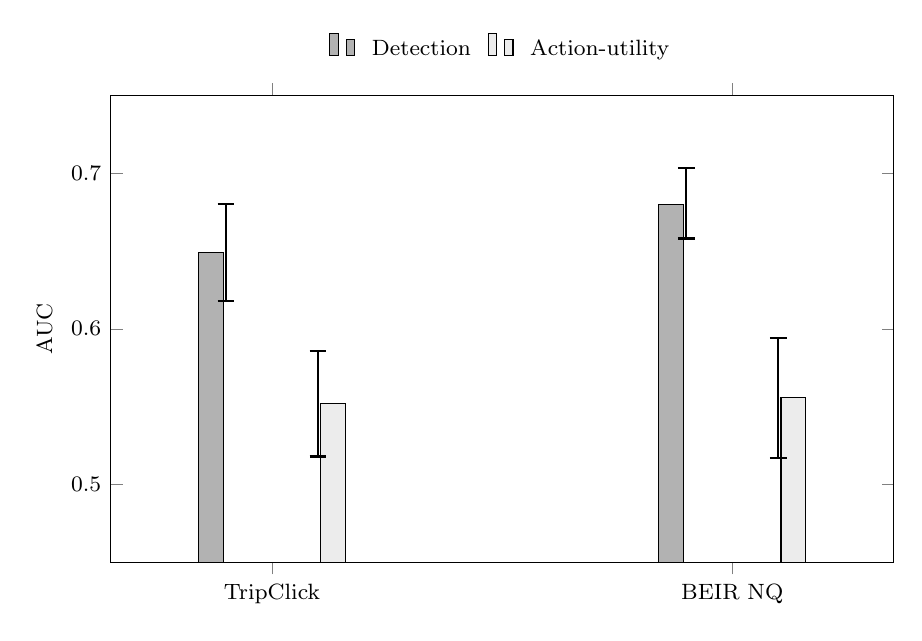
\begin{tikzpicture}
\begin{axis}[
    width=0.95\linewidth,
    height=0.62\linewidth,
    ybar,
    bar width=9pt,
    ymin=0.45, ymax=0.75,
    ylabel={AUC},
    ylabel style={font=\footnotesize},
    xtick={1,3},
    xticklabels={TripClick,BEIR NQ},
    xmin=0.3, xmax=3.7,
    tick label style={font=\footnotesize},
    legend style={font=\footnotesize,draw=none,at={(0.5,1.05)},anchor=south,
        legend columns=2,column sep=4pt},
    axis line style={draw=black},
]
\addplot[fill=gray!60,draw=black] coordinates {(0.8,0.649) (2.8,0.680)};
\addplot[fill=gray!15,draw=black] coordinates {(1.2,0.552) (3.2,0.556)};
\legend{Detection,Action-utility}
\draw[thick] (axis cs:0.8,0.618) -- (axis cs:0.8,0.680);
\draw[thick] (axis cs:0.8,0.618) ++(-3pt,0pt) -- ++(6pt,0pt);
\draw[thick] (axis cs:0.8,0.680) ++(-3pt,0pt) -- ++(6pt,0pt);
\draw[thick] (axis cs:1.2,0.518) -- (axis cs:1.2,0.586);
\draw[thick] (axis cs:1.2,0.518) ++(-3pt,0pt) -- ++(6pt,0pt);
\draw[thick] (axis cs:1.2,0.586) ++(-3pt,0pt) -- ++(6pt,0pt);
\draw[thick] (axis cs:2.8,0.658) -- (axis cs:2.8,0.703);
\draw[thick] (axis cs:2.8,0.658) ++(-3pt,0pt) -- ++(6pt,0pt);
\draw[thick] (axis cs:2.8,0.703) ++(-3pt,0pt) -- ++(6pt,0pt);
\draw[thick] (axis cs:3.2,0.517) -- (axis cs:3.2,0.594);
\draw[thick] (axis cs:3.2,0.517) ++(-3pt,0pt) -- ++(6pt,0pt);
\draw[thick] (axis cs:3.2,0.594) ++(-3pt,0pt) -- ++(6pt,0pt);
\end{axis}
\end{tikzpicture}
\caption{Table~\ref{tab:headline} as bars with 95\% CIs. Detection's
CI is entirely above Action-utility's on both corpora --- the
asymmetry, not just the point estimates, replicates.}
\label{fig:headline}
\end{figure}

\section{Result 2: Does Detection Enable Selective QE?}

The natural response to Result 1 is: detection is hard enough,
fine --- just expand the queries the detector flags as failing. We
test this directly rather than assume it follows.

\begin{table}[h]
\caption{TripClick TAIL test ($n{=}1175$), frozen configuration. Gain
is mean nDCG@10 relative to BM25 alone; NS: 95\% CI crosses zero.}
\label{tab:policies}
\small
\begin{tabular}{@{}lccc@{}}
\toprule
Policy & nDCG@10 & $\Delta$ vs.\ BM25 & \\
\midrule
BM25 & 0.3152 & --- & \\
Static QE & 0.3159 & $+0.0007$ & NS \\
Failure-selective QE & 0.3179 & $+0.0027$ & NS \\
Closed-loop QE & 0.3161 & $+0.0009$ & NS \\
\bottomrule
\end{tabular}
\end{table}

Failure-selective QE's point estimate is the best of the three real
policies --- higher than unconditional Static QE and higher than the
far more expensive closed-loop agent --- while routing only $48.7\%$
of queries to expansion. But none of the three is significantly
different from BM25, and failure-selective QE is not significantly
different from either Static QE or the closed-loop agent directly. The
detector that cleanly separates failing from healthy retrieval
(Result 1) does not, by itself, translate into a selective-expansion
policy that reliably beats doing nothing.

Cost favors the simple policy regardless. The closed-loop agent costs
$24\%$ more generator calls (1.22 vs.\ 0.98 per query) and $36\%$
higher mean latency (15.1s vs.\ 11.1s) than unconditional Static QE
for no significant gain over it. Failure-selective QE, by construction,
invokes the generator on only $48.7\%$ of queries, versus $100\%$ for
both Static QE and the closed-loop agent --- the cheapest of the three
real policies tested is also the one with the best point estimate,
even though none is statistically distinguishable from the others.

\begin{figure}[t]
\centering
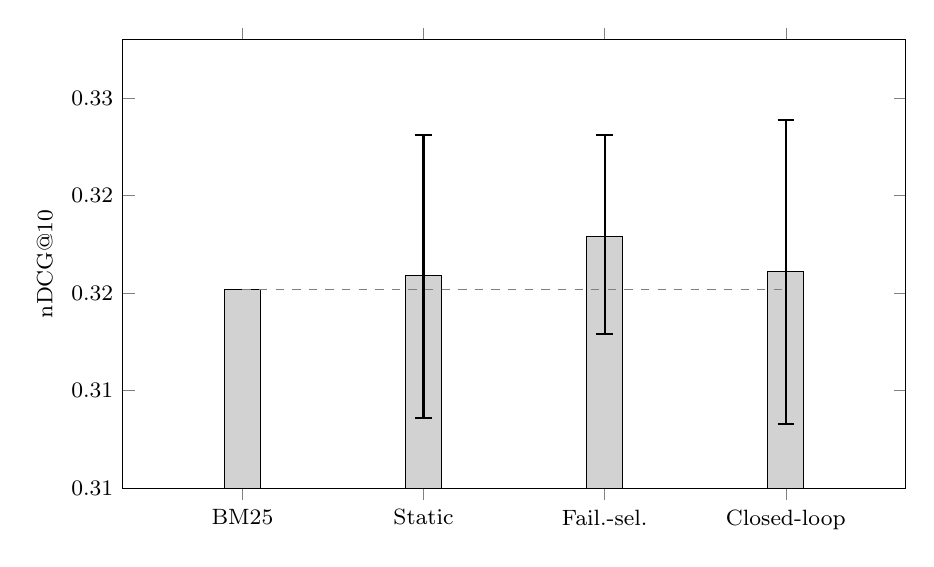
\begin{tikzpicture}
\begin{axis}[
    width=0.95\linewidth,
    height=0.6\linewidth,
    ybar,
    bar width=13pt,
    ymin=0.305, ymax=0.328,
    ylabel={nDCG@10},
    ylabel style={font=\footnotesize},
    symbolic x coords={BM25,Static,Fail.-sel.,Closed-loop},
    xtick=data,
    x tick label style={font=\footnotesize},
    tick label style={font=\footnotesize},
    enlarge x limits=0.22,
    axis line style={draw=black},
]
\addplot[fill=gray!35,draw=black] coordinates
    {(BM25,0.3152) (Static,0.3159) (Fail.-sel.,0.3179) (Closed-loop,0.3161)};
\draw[thick] (axis cs:Static,0.3086) -- (axis cs:Static,0.3231);
\draw[thick] (axis cs:Static,0.3086) ++(-3pt,0pt) -- ++(6pt,0pt);
\draw[thick] (axis cs:Static,0.3231) ++(-3pt,0pt) -- ++(6pt,0pt);
\draw[thick] (axis cs:Fail.-sel.,0.3129) -- (axis cs:Fail.-sel.,0.3231);
\draw[thick] (axis cs:Fail.-sel.,0.3129) ++(-3pt,0pt) -- ++(6pt,0pt);
\draw[thick] (axis cs:Fail.-sel.,0.3231) ++(-3pt,0pt) -- ++(6pt,0pt);
\draw[thick] (axis cs:Closed-loop,0.3083) -- (axis cs:Closed-loop,0.3239);
\draw[thick] (axis cs:Closed-loop,0.3083) ++(-3pt,0pt) -- ++(6pt,0pt);
\draw[thick] (axis cs:Closed-loop,0.3239) ++(-3pt,0pt) -- ++(6pt,0pt);
\draw[dashed,gray] (axis cs:BM25,0.3152) -- (axis cs:Closed-loop,0.3152);
\end{axis}
\end{tikzpicture}
\caption{Table~\ref{tab:policies} as bars (BM25's bar has no error
range, shown as the reference); the other three show the gain's 95\%
CI relative to BM25, translated into absolute nDCG@10. All three
ranges cross BM25's reference line.}
\label{fig:policies}
\end{figure}

\section{Why Selective QE Remains Difficult}

A null policy result is ambiguous: either no benefit exists to select
for, or a selector exists but ours cannot find it. A retrospective
oracle --- per query, the better of BM25 or Static QE under true click
labels, never deployable --- separates these: it gains $+0.0246$
nDCG@10 over BM25 ($p<0.001$), while unconditional Static QE gains only
$+0.0007$. Static QE helps $11.6\%$ of queries and harms $10.6\%$, a
real, roughly balanced mix a perfect selector could exploit. Sweeping
the intervention budget rather than fixing one quota shows this is not
a single unlucky operating point:

\begin{center}
\small
\begin{tabular}{@{}lccc@{}}
\toprule
Quota & Oracle gain & Verifier gain & Verifier \% of oracle \\
\midrule
5\% & $+0.0184$ & $+0.0001$ & $0.5\%$ \\
10\% & $+0.0242$ & $+0.0006$ & $2.5\%$ \\
20\% & $+0.0246$ & $+0.0025$ & $10.2\%$ \\
40\% & $+0.0246$ & $+0.0029$ & $11.8\%$ \\
\bottomrule
\end{tabular}
\end{center}

At every budget below treating every query, the verifier-ranked policy
captures at most $11.8\%$ of the oracle's own gain --- this oracle is
itself susceptible to selection
optimism --- it selects per query using the same sparse click labels
it is evaluated on. Checking the identical oracle definition on TAIL
\emph{validation}, never used to select the oracle itself, shows the
magnitude is split-sensitive on TripClick: $+0.0533$ nDCG@10 there
versus $+0.0246$ on test, non-overlapping CIs, while on NQ the two
nearly agree ($+0.0399$ validation vs.\ $+0.0415$ confirmatory test).
We therefore read the oracle as directional evidence that
heterogeneous, query-specific treatment effects exist, not as a
precise, deployable bound. We checked whether a more formally debiased
estimate is possible from this benchmark rather than assuming it is:
TripClick's public release provides only already-binarized click
labels, even in its ``raw'' qrels, with no underlying click counts or
impression data to bootstrap or split for a repeated-draws correction,
and no independent expert-judgment source (unlike, e.g., TREC DL) to
substitute in its place. A debiased estimate is future work
conditional on access to richer label data this benchmark does not
publicly provide, not a gap we can close with the data at hand. The
evidence as a whole points to
\emph{action-utility prediction}, not the absence of opportunity, as
selective QE's binding constraint.

\textbf{Why the two tasks differ in difficulty.} One plausible
explanation is what each task conditions on. Detection asks a question
about a state that already exists and has already been fully observed:
is \emph{this} ranking, as retrieved, adequate? Action-utility asks a
counterfactual about a state that does not yet exist: would \emph{this
specific}, LLM-generated rewrite have produced a better ranking than
the one already in hand? The second question's target is itself a
high-variance artifact. Decoding is greedy (temperature $0$), so the
generator's output is not stochastic given a fixed input --- the
variance is across \emph{different} queries and evidence, not sampling
noise within one: a deterministic function of (query, evidence) whose
behavior is highly sensitive to evidence the generator did not choose
and may misuse, yielding outputs whose quality is hard to anticipate
from the state that produced them. So even a telemetry vocabulary rich
enough to characterize the current state well need not characterize
the effect of an intervention that state did not determine. This is consistent with Table~\ref{tab:headline}'s
asymmetry despite the action-utility model's richer feature set, and
with why gating signals in general (Section~2) struggle to double as
treatment-effect predictors.

\textbf{Limitations.} The generator is a small, locally hosted 3B-parameter
model under a two-call budget; a larger model might shift either AUC
or the policy comparison. Corpus coverage is two domains, one clinical
and one open-domain; broader coverage remains untested. Click-derived
labels are an imperfect relevance proxy inherited from TripClick.

\section{Conclusion}

Detecting that retrieval has already failed is significantly easier
than predicting whether a specific LLM query-expansion action will fix
it, on two unrelated corpora. As a direct consequence, neither
unconditional QE, a failure-selective controller built on the stronger
detection signal, nor a more expensive closed-loop policy that also
consults post-action telemetry significantly improves a properly-tuned
retriever on ordinary queries. Selective query expansion research
should therefore evaluate intervention-utility prediction directly,
rather than treating query difficulty or retrieval-failure detection
as a proxy for treatment benefit --- the two are empirically different
problems of different difficulty, and conflating them is where
selective QE's promise currently stalls.

\textit{Experimental integrity.} All model, threshold, and retrieval
configuration choices were made on validation data.
Implementation defects surfaced during development were diagnosed from
self-evidently implausible results and fixed before any confirmatory
test evaluation; the complete experimental history, including every
implementation-debugging touch, is documented in the supplementary
repository rather than omitted.

\section*{Ethical Considerations}

All data used (TripClick, BEIR Natural Questions) are existing public
or access-granted research benchmarks, used under their stated
licenses; TripClick's click logs are aggregate, de-identified search
interactions released for non-commercial research, and we do not
attempt to re-identify individual searchers. No new human-subjects
data was collected. The generator is a small, locally hosted model
used only for corpus-grounded query rewriting within a bounded action
space, never for open-ended generation or decisions outside retrieval.
Our central finding --- that detecting retrieval failure is easier
than predicting whether a specific intervention helps --- is a caution
against deploying LLM query expansion (or similar generative
interventions) on the strength of a failure/difficulty detector alone;
we see this as reducing the risk of over-trusting such systems, not
introducing new risk.

\bibliographystyle{ACM-Reference-Format}
\bibliography{references}

\end{document}
